% !TEX root = z_output/_iter_loop_spaces.tex
\documentclass[11pt]{article}
\usepackage{fullpage}
\usepackage{amsmath,amsthm,amssymb}
\usepackage{mathrsfs,nicefrac}
\usepackage{amssymb}
\usepackage{epsfig}
\usepackage[all,2cell]{xy}
\usepackage{sseq}
\usepackage{tocloft}
\usepackage{cancel}
\usepackage[strict]{changepage}
\usepackage{color}
\usepackage{tikz}
\usepackage{extpfeil}
\usepackage{version}
\usepackage{framed}
\definecolor{shadecolor}{rgb}{.925,0.925,0.925}

%\usepackage{ifthen}
%Used for disabling hyperref
\ifx\dontloadhyperref\undefined
%\usepackage[pdftex,pdfborder={0 0 0 [1 1]}]{hyperref}
\usepackage[pdftex,pdfborder={0 0 .5 [1 1]}]{hyperref}
\else
\providecommand{\texorpdfstring}[2]{#1}
\fi
%>>>>>>>>>>>>>>>>>>>>>>>>>>>>>>
%<<<        Versions        <<<
%>>>>>>>>>>>>>>>>>>>>>>>>>>>>>>
%Add in the following line to include all the versions.
%\def\excludeversion#1{\includeversion{#1}}

%>>>>>>>>>>>>>>>>>>>>>>>>>>>>>>
%<<<       Better ToC       <<<
%>>>>>>>>>>>>>>>>>>>>>>>>>>>>>>
\setlength{\cftbeforesecskip}{0.5ex}

%>>>>>>>>>>>>>>>>>>>>>>>>>>>>>>
%<<<      Hyperref mod      <<<
%>>>>>>>>>>>>>>>>>>>>>>>>>>>>>>

%needs more testing
\newcounter{dummyforrefstepcounter}
\newcommand{\labelRIGHTHERE}[1]
{\refstepcounter{dummyforrefstepcounter}\label{#1}}


%>>>>>>>>>>>>>>>>>>>>>>>>>>>>>>
%<<<  Theorem Environments  <<<
%>>>>>>>>>>>>>>>>>>>>>>>>>>>>>>
\ifx\dontloaddefinitionsoftheoremenvironments\undefined
\theoremstyle{plain}
\newtheorem{thm}{Theorem}[section]
\newtheorem*{thm*}{Theorem}
\newtheorem{lem}[thm]{Lemma}
\newtheorem*{lem*}{Lemma}
\newtheorem{prop}[thm]{Proposition}
\newtheorem*{prop*}{Proposition}
\newtheorem{cor}[thm]{Corollary}
\newtheorem*{cor*}{Corollary}
\newtheorem{defprop}[thm]{Definition-Proposition}
\newtheorem*{punchline}{Punchline}
\newtheorem*{conjecture}{Conjecture}
\newtheorem*{claim}{Claim}

\theoremstyle{definition}
\newtheorem{defn}{Definition}[section]
\newtheorem*{defn*}{Definition}
\newtheorem{exmp}{Example}[section]
\newtheorem*{exmp*}{Example}
\newtheorem*{exmps*}{Examples}
\newtheorem*{nonexmp*}{Non-example}
\newtheorem{asspt}{Assumption}[section]
\newtheorem{notation}{Notation}[section]
\newtheorem{exercise}{Exercise}[section]
\newtheorem*{fact*}{Fact}
\newtheorem*{rmk*}{Remark}
\newtheorem{fact}{Fact}
\newtheorem*{aside}{Aside}
\newtheorem*{question}{Question}
\newtheorem*{answer}{Answer}

\else\relax\fi

%>>>>>>>>>>>>>>>>>>>>>>>>>>>>>>
%<<<      Fields, etc.      <<<
%>>>>>>>>>>>>>>>>>>>>>>>>>>>>>>
\DeclareSymbolFont{AMSb}{U}{msb}{m}{n}
\DeclareMathSymbol{\N}{\mathbin}{AMSb}{"4E}
\DeclareMathSymbol{\Octonions}{\mathbin}{AMSb}{"4F}
\DeclareMathSymbol{\Z}{\mathbin}{AMSb}{"5A}
\DeclareMathSymbol{\R}{\mathbin}{AMSb}{"52}
\DeclareMathSymbol{\Q}{\mathbin}{AMSb}{"51}
\DeclareMathSymbol{\PP}{\mathbin}{AMSb}{"50}
\DeclareMathSymbol{\I}{\mathbin}{AMSb}{"49}
\DeclareMathSymbol{\C}{\mathbin}{AMSb}{"43}
\DeclareMathSymbol{\A}{\mathbin}{AMSb}{"41}
\DeclareMathSymbol{\F}{\mathbin}{AMSb}{"46}
\DeclareMathSymbol{\G}{\mathbin}{AMSb}{"47}
\DeclareMathSymbol{\Quaternions}{\mathbin}{AMSb}{"48}


%>>>>>>>>>>>>>>>>>>>>>>>>>>>>>>
%<<<       Operators        <<<
%>>>>>>>>>>>>>>>>>>>>>>>>>>>>>>
\DeclareMathOperator{\ad}{\textbf{ad}}
\DeclareMathOperator{\coker}{coker}
\renewcommand{\ker}{\textup{ker}\,}
\DeclareMathOperator{\End}{End}
\DeclareMathOperator{\Aut}{Aut}
\DeclareMathOperator{\Hom}{Hom}
\DeclareMathOperator{\Maps}{Maps}
\DeclareMathOperator{\Mor}{Mor}
\DeclareMathOperator{\Gal}{Gal}
\DeclareMathOperator{\Ext}{Ext}
\DeclareMathOperator{\Tor}{Tor}
\DeclareMathOperator{\Map}{Map}
\DeclareMathOperator{\Der}{Der}
\DeclareMathOperator{\Rad}{Rad}
\DeclareMathOperator{\rank}{rank}
\DeclareMathOperator{\ArfInvariant}{Arf}
\DeclareMathOperator{\KervaireInvariant}{Ker}
\DeclareMathOperator{\im}{im}
\DeclareMathOperator{\coim}{coim}
\DeclareMathOperator{\trace}{tr}
\DeclareMathOperator{\supp}{supp}
\DeclareMathOperator{\ann}{ann}
\DeclareMathOperator{\spec}{Spec}
\DeclareMathOperator{\SPEC}{\textbf{Spec}}
\DeclareMathOperator{\proj}{Proj}
\DeclareMathOperator{\PROJ}{\textbf{Proj}}
\DeclareMathOperator{\fiber}{F}
\DeclareMathOperator{\cofiber}{C}
\DeclareMathOperator{\cone}{cone}
\DeclareMathOperator{\skel}{sk}
\DeclareMathOperator{\coskel}{cosk}
\DeclareMathOperator{\conn}{conn}
\DeclareMathOperator{\colim}{colim}
\DeclareMathOperator{\limit}{lim}
\DeclareMathOperator{\ch}{ch}
\DeclareMathOperator{\Vect}{Vect}
\DeclareMathOperator{\GrthGrp}{GrthGp}
\DeclareMathOperator{\Sym}{Sym}
\DeclareMathOperator{\Prob}{\mathbb{P}}
\DeclareMathOperator{\Exp}{\mathbb{E}}
\DeclareMathOperator{\GeomMean}{\mathbb{G}}
\DeclareMathOperator{\Var}{Var}
\DeclareMathOperator{\Cov}{Cov}
\DeclareMathOperator{\Sp}{Sp}
\DeclareMathOperator{\Seq}{Seq}
\DeclareMathOperator{\Cyl}{Cyl}
\DeclareMathOperator{\Ev}{Ev}
\DeclareMathOperator{\sh}{sh}
\DeclareMathOperator{\intHom}{\underline{Hom}}
\DeclareMathOperator{\Frac}{frac}



%>>>>>>>>>>>>>>>>>>>>>>>>>>>>>>
%<<<   Cohomology Theories  <<<
%>>>>>>>>>>>>>>>>>>>>>>>>>>>>>>
\DeclareMathOperator{\KR}{{K\R}}
\DeclareMathOperator{\KO}{{KO}}
\DeclareMathOperator{\K}{{K}}
\DeclareMathOperator{\OmegaO}{{\Omega_{\Octonions}}}

%>>>>>>>>>>>>>>>>>>>>>>>>>>>>>>
%<<<   Algebraic Geometry   <<<
%>>>>>>>>>>>>>>>>>>>>>>>>>>>>>>
\DeclareMathOperator{\Spec}{Spec}
\DeclareMathOperator{\Proj}{Proj}
\DeclareMathOperator{\Sing}{Sing}
\DeclareMathOperator{\shfHom}{\mathscr{H}\textit{\!\!om}}
\DeclareMathOperator{\WeilDivisors}{{Div}}
\DeclareMathOperator{\CartierDivisors}{{CaDiv}}
\DeclareMathOperator{\PrincipalWeilDivisors}{{PrDiv}}
\DeclareMathOperator{\LocallyPrincipalWeilDivisors}{{LPDiv}}
\DeclareMathOperator{\PrincipalCartierDivisors}{{PrCaDiv}}
\DeclareMathOperator{\DivisorClass}{{Cl}}
\DeclareMathOperator{\CartierClass}{{CaCl}}
\DeclareMathOperator{\Picard}{{Pic}}
\DeclareMathOperator{\Frob}{Frob}


%>>>>>>>>>>>>>>>>>>>>>>>>>>>>>>
%<<<  Mathematical Objects  <<<
%>>>>>>>>>>>>>>>>>>>>>>>>>>>>>>
\newcommand{\sll}{\mathfrak{sl}}
\newcommand{\gl}{\mathfrak{gl}}
\newcommand{\GL}{\mbox{GL}}
\newcommand{\PGL}{\mbox{PGL}}
\newcommand{\SL}{\mbox{SL}}
\newcommand{\Mat}{\mbox{Mat}}
\newcommand{\Gr}{\textup{Gr}}
\newcommand{\Squ}{\textup{Sq}}
\newcommand{\catSet}{\textit{Sets}}
\newcommand{\RP}{{\R\PP}}
\newcommand{\CP}{{\C\PP}}
\newcommand{\Steen}{\mathscr{A}}
\newcommand{\Orth}{\textup{\textbf{O}}}

%>>>>>>>>>>>>>>>>>>>>>>>>>>>>>>
%<<<  Mathematical Symbols  <<<
%>>>>>>>>>>>>>>>>>>>>>>>>>>>>>>
\newcommand{\DASH}{\textup{---}}
\newcommand{\op}{\textup{op}}
\newcommand{\CW}{\textup{CW}}
\newcommand{\ob}{\textup{ob}\,}
\newcommand{\ho}{\textup{ho}}
\newcommand{\st}{\textup{st}}
\newcommand{\id}{\textup{id}}
\newcommand{\Bullet}{\ensuremath{\bullet} }
\newcommand{\sprod}{\wedge}

%>>>>>>>>>>>>>>>>>>>>>>>>>>>>>>
%<<<      Some Arrows       <<<
%>>>>>>>>>>>>>>>>>>>>>>>>>>>>>>
\newcommand{\nt}{\Longrightarrow}
\let\shortmapsto\mapsto
\let\mapsto\longmapsto
\newcommand{\mapsfrom}{\,\reflectbox{$\mapsto$}\ }
\newcommand{\bigrightsquig}{\scalebox{2}{\ensuremath{\rightsquigarrow}}}
\newcommand{\bigleftsquig}{\reflectbox{\scalebox{2}{\ensuremath{\rightsquigarrow}}}}

%\newcommand{\cofibration}{\xhookrightarrow{\phantom{\ \,{\sim\!}\ \ }}}
%\newcommand{\fibration}{\xtwoheadrightarrow{\phantom{\sim\!}}}
%\newcommand{\acycliccofibration}{\xhookrightarrow{\ \,{\sim\!}\ \ }}
%\newcommand{\acyclicfibration}{\xtwoheadrightarrow{\sim\!}}
%\newcommand{\leftcofibration}{\xhookleftarrow{\phantom{\ \,{\sim\!}\ \ }}}
%\newcommand{\leftfibration}{\xtwoheadleftarrow{\phantom{\sim\!}}}
%\newcommand{\leftacycliccofibration}{\xhookleftarrow{\ \ {\sim\!}\,\ }}
%\newcommand{\leftacyclicfibration}{\xtwoheadleftarrow{\sim\!}}
%\newcommand{\weakequiv}{\xrightarrow{\ \,\sim\,\ }}
%\newcommand{\leftweakequiv}{\xleftarrow{\ \,\sim\,\ }}

\newcommand{\cofibration}
{\xhookrightarrow{\phantom{\ \,{\raisebox{-.3ex}[0ex][0ex]{\scriptsize$\sim$}\!}\ \ }}}
\newcommand{\fibration}
{\xtwoheadrightarrow{\phantom{\raisebox{-.3ex}[0ex][0ex]{\scriptsize$\sim$}\!}}}
\newcommand{\acycliccofibration}
{\xhookrightarrow{\ \,{\raisebox{-.55ex}[0ex][0ex]{\scriptsize$\sim$}\!}\ \ }}
\newcommand{\acyclicfibration}
{\xtwoheadrightarrow{\raisebox{-.6ex}[0ex][0ex]{\scriptsize$\sim$}\!}}
\newcommand{\leftcofibration}
{\xhookleftarrow{\phantom{\ \,{\raisebox{-.3ex}[0ex][0ex]{\scriptsize$\sim$}\!}\ \ }}}
\newcommand{\leftfibration}
{\xtwoheadleftarrow{\phantom{\raisebox{-.3ex}[0ex][0ex]{\scriptsize$\sim$}\!}}}
\newcommand{\leftacycliccofibration}
{\xhookleftarrow{\ \ {\raisebox{-.55ex}[0ex][0ex]{\scriptsize$\sim$}\!}\,\ }}
\newcommand{\leftacyclicfibration}
{\xtwoheadleftarrow{\raisebox{-.6ex}[0ex][0ex]{\scriptsize$\sim$}\!}}
\newcommand{\weakequiv}
{\xrightarrow{\ \,\raisebox{-.3ex}[0ex][0ex]{\scriptsize$\sim$}\,\ }}
\newcommand{\leftweakequiv}
{\xleftarrow{\ \,\raisebox{-.3ex}[0ex][0ex]{\scriptsize$\sim$}\,\ }}

%>>>>>>>>>>>>>>>>>>>>>>>>>>>>>>
%<<<    xymatrix Arrows     <<<
%>>>>>>>>>>>>>>>>>>>>>>>>>>>>>>
\newdir{ >}{{}*!/-5pt/@{>}}
\newcommand{\xycof}{\ar@{ >->}}
\newcommand{\xycofib}{\ar@{^{(}->}}
\newcommand{\xycofibdown}{\ar@{_{(}->}}
\newcommand{\xyfib}{\ar@{->>}}
\newcommand{\xymapsto}{\ar@{|->}}

%>>>>>>>>>>>>>>>>>>>>>>>>>>>>>>
%<<<     Greek Letters      <<<
%>>>>>>>>>>>>>>>>>>>>>>>>>>>>>>
%\newcommand{\oldphi}{\phi}
%\renewcommand{\phi}{\varphi}
\let\oldphi\phi
\let\phi\varphi
\renewcommand{\to}{\longrightarrow}
\newcommand{\from}{\longleftarrow}
\newcommand{\eps}{\varepsilon}

%>>>>>>>>>>>>>>>>>>>>>>>>>>>>>>
%<<<  1st-4th & parentheses <<<
%>>>>>>>>>>>>>>>>>>>>>>>>>>>>>>
\newcommand{\first}{^\text{st}}
\newcommand{\second}{^\text{nd}}
\newcommand{\third}{^\text{rd}}
\newcommand{\fourth}{^\text{th}}
\newcommand{\ZEROTH}{$0^\text{th}$ }
\newcommand{\FIRST}{$1^\text{st}$ }
\newcommand{\SECOND}{$2^\text{nd}$ }
\newcommand{\THIRD}{$3^\text{rd}$ }
\newcommand{\FOURTH}{$4^\text{th}$ }
\newcommand{\iTH}{$i^\text{th}$ }
\newcommand{\jTH}{$j^\text{th}$ }
\newcommand{\nTH}{$n^\text{th}$ }

%>>>>>>>>>>>>>>>>>>>>>>>>>>>>>>
%<<<    upright commands    <<<
%>>>>>>>>>>>>>>>>>>>>>>>>>>>>>>
\newcommand{\upcol}{\textup{:}}
\newcommand{\upsemi}{\textup{;}}
\providecommand{\lparen}{\textup{(}}
\providecommand{\rparen}{\textup{)}}
\renewcommand{\lparen}{\textup{(}}
\renewcommand{\rparen}{\textup{)}}
\newcommand{\Iff}{\emph{iff} }

%>>>>>>>>>>>>>>>>>>>>>>>>>>>>>>
%<<<     Environments       <<<
%>>>>>>>>>>>>>>>>>>>>>>>>>>>>>>
\newcommand{\squishlist}
{ %\setlength{\topsep}{100pt} doesn't seem to do anything.
  \setlength{\itemsep}{.5pt}
  \setlength{\parskip}{0pt}
  \setlength{\parsep}{0pt}}
\newenvironment{itemise}{
\begin{list}{\textup{$\rightsquigarrow$}}
   {  \setlength{\topsep}{1mm}
      \setlength{\itemsep}{1pt}
      \setlength{\parskip}{0pt}
      \setlength{\parsep}{0pt}
   }
}{\end{list}\vspace{-.1cm}}
\newcommand{\INDENT}{\textbf{}\phantom{space}}
\renewcommand{\INDENT}{\rule{.7cm}{0cm}}

\newcommand{\itm}[1][$\rightsquigarrow$]{\item[{\makebox[.5cm][c]{\textup{#1}}}]}


%\newcommand{\rednote}[1]{{\color{red}#1}\makebox[0cm][l]{\scalebox{.1}{rednote}}}
%\newcommand{\bluenote}[1]{{\color{blue}#1}\makebox[0cm][l]{\scalebox{.1}{rednote}}}

\newcommand{\rednote}[1]
{{\color{red}#1}\makebox[0cm][l]{\scalebox{.1}{\rotatebox{90}{?????}}}}
\newcommand{\bluenote}[1]
{{\color{blue}#1}\makebox[0cm][l]{\scalebox{.1}{\rotatebox{90}{?????}}}}


\newcommand{\funcdef}[4]{\begin{align*}
#1&\to #2\\
#3&\mapsto#4
\end{align*}}

%\newcommand{\comment}[1]{}

%>>>>>>>>>>>>>>>>>>>>>>>>>>>>>>
%<<<       Categories       <<<
%>>>>>>>>>>>>>>>>>>>>>>>>>>>>>>
\newcommand{\Ens}{{\mathscr{E}ns}}
\DeclareMathOperator{\Sheaves}{{\mathsf{Shf}}}
\DeclareMathOperator{\Presheaves}{{\mathsf{PreShf}}}
\DeclareMathOperator{\Psh}{{\mathsf{Psh}}}
\DeclareMathOperator{\Shf}{{\mathsf{Shf}}}
\DeclareMathOperator{\Varieties}{{\mathsf{Var}}}
\DeclareMathOperator{\Schemes}{{\mathsf{Sch}}}
\DeclareMathOperator{\Rings}{{\mathsf{Rings}}}
\DeclareMathOperator{\AbGp}{{\mathsf{AbGp}}}
\DeclareMathOperator{\Modules}{{\mathsf{\!-Mod}}}
\DeclareMathOperator{\fgModules}{{\mathsf{\!-Mod}^{\textup{fg}}}}
\DeclareMathOperator{\QuasiCoherent}{{\mathsf{QCoh}}}
\DeclareMathOperator{\Coherent}{{\mathsf{Coh}}}
\DeclareMathOperator{\GSW}{{\mathcal{SW}^G}}
\DeclareMathOperator{\Burnside}{{\mathsf{Burn}}}
\DeclareMathOperator{\GSet}{{G\mathsf{Set}}}
\DeclareMathOperator{\FinGSet}{{G\mathsf{Set}^\textup{fin}}}
\DeclareMathOperator{\HSet}{{H\mathsf{Set}}}
\DeclareMathOperator{\Cat}{{\mathsf{Cat}}}
\DeclareMathOperator{\Fun}{{\mathsf{Fun}}}
\DeclareMathOperator{\Orb}{{\mathsf{Orb}}}
\DeclareMathOperator{\Set}{{\mathsf{Set}}}
\DeclareMathOperator{\sSet}{{\mathsf{sSet}}}
\DeclareMathOperator{\Top}{{\mathsf{Top}}}
\DeclareMathOperator{\GSpectra}{{G-\mathsf{Spectra}}}
\DeclareMathOperator{\Lan}{Lan}
\DeclareMathOperator{\Ran}{Ran}

%>>>>>>>>>>>>>>>>>>>>>>>>>>>>>>
%<<<     Script Letters     <<<
%>>>>>>>>>>>>>>>>>>>>>>>>>>>>>>
\newcommand{\scrQ}{\mathscr{Q}}
\newcommand{\scrW}{\mathscr{W}}
\newcommand{\scrE}{\mathscr{E}}
\newcommand{\scrR}{\mathscr{R}}
\newcommand{\scrT}{\mathscr{T}}
\newcommand{\scrY}{\mathscr{Y}}
\newcommand{\scrU}{\mathscr{U}}
\newcommand{\scrI}{\mathscr{I}}
\newcommand{\scrO}{\mathscr{O}}
\newcommand{\scrP}{\mathscr{P}}
\newcommand{\scrA}{\mathscr{A}}
\newcommand{\scrS}{\mathscr{S}}
\newcommand{\scrD}{\mathscr{D}}
\newcommand{\scrF}{\mathscr{F}}
\newcommand{\scrG}{\mathscr{G}}
\newcommand{\scrH}{\mathscr{H}}
\newcommand{\scrJ}{\mathscr{J}}
\newcommand{\scrK}{\mathscr{K}}
\newcommand{\scrL}{\mathscr{L}}
\newcommand{\scrZ}{\mathscr{Z}}
\newcommand{\scrX}{\mathscr{X}}
\newcommand{\scrC}{\mathscr{C}}
\newcommand{\scrV}{\mathscr{V}}
\newcommand{\scrB}{\mathscr{B}}
\newcommand{\scrN}{\mathscr{N}}
\newcommand{\scrM}{\mathscr{M}}

%>>>>>>>>>>>>>>>>>>>>>>>>>>>>>>
%<<<     Fractur Letters    <<<
%>>>>>>>>>>>>>>>>>>>>>>>>>>>>>>
\newcommand{\frakQ}{\mathfrak{Q}}
\newcommand{\frakW}{\mathfrak{W}}
\newcommand{\frakE}{\mathfrak{E}}
\newcommand{\frakR}{\mathfrak{R}}
\newcommand{\frakT}{\mathfrak{T}}
\newcommand{\frakY}{\mathfrak{Y}}
\newcommand{\frakU}{\mathfrak{U}}
\newcommand{\frakI}{\mathfrak{I}}
\newcommand{\frakO}{\mathfrak{O}}
\newcommand{\frakP}{\mathfrak{P}}
\newcommand{\frakA}{\mathfrak{A}}
\newcommand{\frakS}{\mathfrak{S}}
\newcommand{\frakD}{\mathfrak{D}}
\newcommand{\frakF}{\mathfrak{F}}
\newcommand{\frakG}{\mathfrak{G}}
\newcommand{\frakH}{\mathfrak{H}}
\newcommand{\frakJ}{\mathfrak{J}}
\newcommand{\frakK}{\mathfrak{K}}
\newcommand{\frakL}{\mathfrak{L}}
\newcommand{\frakZ}{\mathfrak{Z}}
\newcommand{\frakX}{\mathfrak{X}}
\newcommand{\frakC}{\mathfrak{C}}
\newcommand{\frakV}{\mathfrak{V}}
\newcommand{\frakB}{\mathfrak{B}}
\newcommand{\frakN}{\mathfrak{N}}
\newcommand{\frakM}{\mathfrak{M}}

\newcommand{\frakq}{\mathfrak{q}}
\newcommand{\frakw}{\mathfrak{w}}
\newcommand{\frake}{\mathfrak{e}}
\newcommand{\frakr}{\mathfrak{r}}
\newcommand{\frakt}{\mathfrak{t}}
\newcommand{\fraky}{\mathfrak{y}}
\newcommand{\fraku}{\mathfrak{u}}
\newcommand{\fraki}{\mathfrak{i}}
\newcommand{\frako}{\mathfrak{o}}
\newcommand{\frakp}{\mathfrak{p}}
\newcommand{\fraka}{\mathfrak{a}}
\newcommand{\fraks}{\mathfrak{s}}
\newcommand{\frakd}{\mathfrak{d}}
\newcommand{\frakf}{\mathfrak{f}}
\newcommand{\frakg}{\mathfrak{g}}
\newcommand{\frakh}{\mathfrak{h}}
\newcommand{\frakj}{\mathfrak{j}}
\newcommand{\frakk}{\mathfrak{k}}
\newcommand{\frakl}{\mathfrak{l}}
\newcommand{\frakz}{\mathfrak{z}}
\newcommand{\frakx}{\mathfrak{x}}
\newcommand{\frakc}{\mathfrak{c}}
\newcommand{\frakv}{\mathfrak{v}}
\newcommand{\frakb}{\mathfrak{b}}
\newcommand{\frakn}{\mathfrak{n}}
\newcommand{\frakm}{\mathfrak{m}}

%>>>>>>>>>>>>>>>>>>>>>>>>>>>>>>
%<<<  Caligraphic Letters   <<<
%>>>>>>>>>>>>>>>>>>>>>>>>>>>>>>
\newcommand{\calQ}{\mathcal{Q}}
\newcommand{\calW}{\mathcal{W}}
\newcommand{\calE}{\mathcal{E}}
\newcommand{\calR}{\mathcal{R}}
\newcommand{\calT}{\mathcal{T}}
\newcommand{\calY}{\mathcal{Y}}
\newcommand{\calU}{\mathcal{U}}
\newcommand{\calI}{\mathcal{I}}
\newcommand{\calO}{\mathcal{O}}
\newcommand{\calP}{\mathcal{P}}
\newcommand{\calA}{\mathcal{A}}
\newcommand{\calS}{\mathcal{S}}
\newcommand{\calD}{\mathcal{D}}
\newcommand{\calF}{\mathcal{F}}
\newcommand{\calG}{\mathcal{G}}
\newcommand{\calH}{\mathcal{H}}
\newcommand{\calJ}{\mathcal{J}}
\newcommand{\calK}{\mathcal{K}}
\newcommand{\calL}{\mathcal{L}}
\newcommand{\calZ}{\mathcal{Z}}
\newcommand{\calX}{\mathcal{X}}
\newcommand{\calC}{\mathcal{C}}
\newcommand{\calV}{\mathcal{V}}
\newcommand{\calB}{\mathcal{B}}
\newcommand{\calN}{\mathcal{N}}
\newcommand{\calM}{\mathcal{M}}

%>>>>>>>>>>>>>>>>>>>>>>>>>>>>>>
%<<<<<<<<<DEPRECIATED<<<<<<<<<<
%>>>>>>>>>>>>>>>>>>>>>>>>>>>>>>

%%% From Kac's template
% 1-inch margins, from fullpage.sty by H.Partl, Version 2, Dec. 15, 1988.
%\topmargin 0pt
%\advance \topmargin by -\headheight
%\advance \topmargin by -\headsep
%\textheight 9.1in
%\oddsidemargin 0pt
%\evensidemargin \oddsidemargin
%\marginparwidth 0.5in
%\textwidth 6.5in
%
%\parindent 0in
%\parskip 1.5ex
%%\renewcommand{\baselinestretch}{1.25}

%%% From the net
%\newcommand{\pullbackcorner}[1][dr]{\save*!/#1+1.2pc/#1:(1,-1)@^{|-}\restore}
%\newcommand{\pushoutcorner}[1][dr]{\save*!/#1-1.2pc/#1:(-1,1)@^{|-}\restore}









\newcommand{\Aff}{\textup{Aff}}

%\def\excludeversion#1{\includeversion{#1}}
\excludeversion{chapter1-3}
\includeversion{chapter4-6}
\excludeversion{chapter7-9}

\title{The Geometry of Iterated Loop Spaces\small{ --- J.\ P.\ May}}

\newcommand{\labsq}[6][0]{
\draw (#2+#1,#3)--(#4+#1,#3)--(#4+#1,#5)--(#2+#1,#5)-- cycle;
\path (.5*#2+.5*#4+#1,.5*#3+.5*#5) node[font=\scriptsize] {#6};
}
\begin{document}
%\tableofcontents
\begin{chapter1-3}
\section{Operads and \texorpdfstring{$\scrC$}{C}-spaces}
Let $\scrU$ be the category of compactly generated Hausdorff spaces and continuous
 maps. 
Let $\scrT$ be the same with nondegenerate basepoints.

An \emph{operad} $\scrC$ consists of spaces $\scrC(j)\in\scrU$ for $j\geq0$,
 with $\scrC(0)=*$, and maps
\[\gamma:\scrC(k)\times\scrC(j_1)\times\cdots\times\scrC(j_k)\to\scrC(j)
\text{ whenever }j=\sum j_i,\]
subject to certain restrictions. We should interpret the points of $\scrC(j)$ as
$j$-adic operations, and the restrictions reflect this interpretation.
$\gamma(c;d_1,\ldots,d_k)$ should be viewed as the operation which takes $j$
inputs, applies $d_1,\ldots,d_k$ to them in order, and then hits the list of
results with $c$.
\begin{itemise}
\item An associativity formula holds.
\item There's an identity $1\in\scrC(1)$ such that $\gamma(c;1^k)=c$ for all $c$.
\item There's a right action of $\Sigma_j$ on $\scrC(j)$ which should be viewed as
permutation of the arguments of an operation. There's an equivariance formula on
the function $\gamma$. An operad is $\Sigma$-free is $\Sigma_j$ acts freely for
each $j$. The equivariance formulae are:
\[\gamma(c\sigma;d_1,\ldots,d_k)=\gamma(c;d_{\sigma^{-1}1},\ldots,
d_{\sigma^{-1}k})\sigma'\text{ where }\sigma'\text{ acts in 
blocks of size $|d_i|$}.\]
\[\gamma(c;d_1\tau_1,\ldots,d_k\tau_k)=\gamma(c;d_1,\ldots,d_k)(\tau_1\oplus
\cdots\oplus\tau_k).\]
\end{itemise}
A morphism of operads is the only thing it could be. The \emph{endomorphism
operad} $\xi_X$ of $X\in\scrT$ has $\xi_X(j)$ the space of based maps $X^j\to
X$, with the only operad structure it could have. The axioms for an operad are
modelled on the obvious properties of $\xi_X$.

An operation $\theta$ of an operad $\scrC$ on a space is a morphism
$\theta:\scrC\to\xi_X$, and $(X,\theta)$ is then said to be a $\scrC$-space. These
form a category $\scrC[\scrT]$, whose morphisms consist of maps in $\scrT$ which
commute with the action.
\begin{thm*}[1.3]
There exist $\Sigma$-free operads $\scrC_n$ ($1\leq n\leq\infty$) such that every
$n$-fold loop space is a $\scrC_n$-space, and every connected $\scrC_n$-space
is weakly equivalent to an $n$-fold loop space. (The spaces $\scrC_n(j)$ are 
$(n-2)$-connected).
\end{thm*}
When $n=1$  (resp.\ $n=\infty$), $\scrC_1$ can be any $A_\infty$ 
(resp.\ $E_\infty$) operad, as defined later.

Let $\scrC$ be any operad and $X$ a $\scrC$-space. For any point
$c\in\scrC(1)$, $\theta_2(c):X^2\to X$ is a candidate multiplication.
Now if $\scrC(1)$ is connected, then $*$ is a two-sided homotopy identity, as
we can use any paths from $\gamma(c;1,*)$ to $1$, etc.
If moreover $\Sigma_2$ is connected, using the transposition we have that
$\theta_2(c)$ is homotopy commutative.

Note that Stasheff's $A_\infty$-space theory states that an $H$-space is of
the homotopy type of a loop space \Iff it has all possible higher coherence
homotopies for associativity.
\begin{lem*}[1.4]
An action $\theta:\scrC\to\xi_X$ determines and is determined by maps 
$\theta_j:\scrC(j)\times X^j\to X$ (adjoint to the maps $\scrC(j)\to\xi_X(j)$)
satisfying some coherences and equivariances, and morphisms of $\scrC$-spaces 
can be easily described in this language.
\end{lem*}
\begin{lem*}[1.5]
If $X\in\scrC[\scrT]$, and $(Y,A)$ is an NDR-pair in $\scrU$, then 
$\Map((Y,A),(X,*))=:X^{(Y,A)}$ is also a $\scrC$-space. (Note that operations
on $X$ give rise to operations on $X^{(Y,A)}$). In particular, $\scrC[\scrT]$ is
closed under taking path and loop spaces.
\end{lem*}
\begin{lem*}[1.6]
The one point space $*$ is a zero object in $\scrC[\scrT]$.
\end{lem*}
\begin{lem*}[1.7]
Given maps $X\to B$ and $Y\to B$ of $\scrC$-spaces, the fibre product is a 
$\scrC$-space, and is the fibre product in the category $\scrC[\scrT]$.
\end{lem*}
\begin{lem*}[1.8] We get a bunch of nice $\scrC$-morphisms from a $\scrC$-morphism
$X\to Y$ by taking a homotopy fibre-type diagram:
\[\xymatrix{
\makebox[2cm][r]{$\widetilde X=X\times_Y(Y^I)$}\ar[r]\ar[d]&Y^I\ar[d]\\
X\ar[r]&Y
}\]
In particular, we get an inclusion $i:X\to \widetilde X$,
retraction $r:\widetilde X\to X$, and fibration 
$\widetilde f:\widetilde X\to Y$.
\end{lem*}
\begin{lem*}[1.9]
Suppose $X\in\scrC[\scrT]$, and $c\in\scrC(2)$ is fixed, giving 
$\oldphi:=\theta(c):X^2\to X$. Let 
$\oldphi_j=\oldphi(1\times \oldphi_{j-1}):X^j\to X$ be the iterated product 
for each $j$.
\begin{itemise}
\item If $\scrC(j)$ is connected and $d\in\scrC(j)$, then $\theta(d)$ is 
homotopic to the iterated product $\oldphi_j$.
\item If $\scrC(j)$ is $\Sigma_j$-free and $\scrC(2j)$ is contractible, then given
$2j$ points of $X$ and a point $d\in\scrC(j)$, it is equivalent to either ``first
multiply the points in pairs using $\oldphi$, then apply $\theta(d)$'', or to apply 
$\theta(d)$ to the points in groups of $d$, and the multiply the results with
$\oldphi$. More precisely, the following is $\Sigma_j$-equivariantly homotopy
commutative:
\[\xymatrix@C=3cm{\scrC(j)\times(X\times X)^j
\ar[r]^{(\theta\times\theta)_j}\ar[d]^{1\times\oldphi^j}&X\times X\ar[d]^\oldphi\\
\scrC(j)\times X\ar[r]^{\theta_j}&X
}\]
\end{itemise}
\end{lem*}
\section{Operads and monads}
A monad $(C,\mu,\eta)$ in a category $\scrT$ is to be a monoid object in the category of endofunctors on $\scrT$. Explicitly, $C:\scrT\to\scrT$ is an endofunctor, and $\mu:C^2\to C$ and $\eta:1\to C$ are natural transformations such that:
\[\xymatrix@C=1.5cm{
CX\ar[r]^{C(\eta_X)}&CCX\ar[d]_{\mu_X}&CX\ar[l]_{\eta_{CX}}\\
&CX\ar@{=}[lu]\ar@{=}[ru]
}
\text{ and }
\xymatrix@C=1.5cm{
CCCX\ar[r]^{\mu_{CX}}\ar[d]_{C(\mu_X)}&CCX\ar[d]_{\mu_X}\\
CCX\ar[r]^{\mu_X}&CX
}
\]
If $\psi$ is a natural transformation $C\to C'$, we can define
$\psi^2:C^2\to (C')^2$ via either composite:
\[\xymatrix@C=1.5cm{
C^2X\ar[d]_{\psi_{CX}}\ar[r]^{C(\psi_X)}&CC'X\ar[d]^{\psi_{C'X}}\\
C'CX\ar[r]^{C'(\psi_X)}&(C')^2X
}\]
Then a morphism of monads is a natural transformation compatible with unit and
multiplication.

An algebra over a monad $C$ is an object $X\in\scrT$ with a map $\xi:CX\to X$
such that
\[\xymatrix{
X\ar[r]^\eta&CX\ar[d]\\
&X\ar@{=}[lu]
}\raisebox{-.67cm}{\text{ and }}
\xymatrix{
CCX\ar[r]^\mu\ar[d]^{c\xi}&CX\ar[d]_\xi\\
CX\ar[r]^\xi&X
}\]
The category of $C$-algebras and morphisms is denoted $C[\scrT]$.

\subsection{Constructing a monad from an operad}
Given an operad $\scrC$, there are maps $\sigma_i:\scrC(j)\to\scrC(j-1)$ for
$0\leq i<j$, essentially defined by substituting the basepoint in the \iTH
argument. That is by setting:
\[\sigma_ic:=\gamma(c;s_i)\text{ where }s_i:=(1,\cdots,1,*,1,\cdots,1)\in \scrC(1)^i\times \scrC(0)\times\scrC(1)^{j-(i+1)}.\]
We can construct the monad associated to an operad $\scrC$ as follows. For any
$X\in\scrT$, define $CX:=\coprod_{j\geq0}\scrC(j)\times X^j/\approx$, where
$\approx$ is the relation generated by:
\begin{itemise}
\item $(\sigma_ic,y)\approx (c,s_iy)$ \ (for $y\in X^{j-1}$ and $c\in \scrC(j)$); and
\item $(c\sigma,y)\approx (c,\sigma y)$ \ (for $y\in X^{j}$, $c\in \scrC(j)$, and $\sigma\in\Sigma_j$).
\end{itemise}
The set $CX$ might be viewed as the set of all images $c(y)$ of $y\in X^j$ under $c\in\scrC(j)$ in an arbitrary action of $\scrC$. All we know about an arbitrary action is encoded in the above two relations.


An element of $CCX$ consists of $c\in \scrC(k)$ and $k$ elements 
$(d_s,y_s)\in \scrC(j_s)\times X^{j_s}$. Now we could always sub the $d_s$
into $c$, which gives us the multiplication $\mu$ in our monad. That is:
\[\mu:CCX\to CX\text{ defined by }
\mu[c,([d_i,y_i])_{i=1}^{|c|}]:=[\gamma(c;(d_i)),(y_i)].\]
Of course, $\eta:X\to CX$ is nothing but $x\mapsto [1,x]$.

If $\pi\subset\Sigma_j$, 
and $\pi$ acts on $W\in\scrU$ from the right, we get a space:
\[e(W,\pi,X):=W_+\wedge_\pi X^{[j]}.\]
Now $CX$ is filtered by $F_kCX$, the image of
$\coprod_{j\leq k}\scrC(j)\times X^j$ in $CX$. We give the $F_kCX$ the quotient topology, and $CX$ the direct limit topology.
\begin{prop*}[2.6]
The inclusions
$F_{k-1}\subseteq F_{k}$ are cofibrations, and $F_{k}/F_{k-1}=e[\scrC(j),\Sigma_j,X]$. Moreover, $C$ is a limit and homotopy preserving
functor.
\end{prop*}
Now the $CX$ are in fact $\scrC$-spaces, and:
\begin{thm*}[2.7 --- Approximation]
For the operads $\scrC_n$, there's a natural map of $\scrC$-spaces
$\alpha_n:C_nX\to\Omega^n\Sigma^nX$, which is a weak equivalence if $X$
is connected. In fact, $\Omega^n\Sigma^n$ is a monad, and 
$\alpha_n:C_n\to\Omega^n\Sigma^n$ is a map of monads.
\end{thm*}
\noindent
Note that the reason $\Omega^n\Sigma^n$ is a monad is that $F=\Sigma^n$
and $G=\Omega^n$ are adjoint functors, and thus $GF$ is a monad, whose unit is
the unit of the adjunction, and whose multiplication is $G\epsilon F$, where
$\epsilon$ is the counit of the adjunction. The unit-counit identities ensure
that $\mu$ and $\eta$ are compatible.
\begin{prop*}[2.8]
There's a 1-1 correspondence between $\scrC$-actions $\scrC\to\xi_X$ and 
$C$-algebra structure maps $\xi:CX\to X$, giving an equivalence of categories 
$\scrC[\scrT]\simeq C[\scrT]$. Here $\theta$ corresponds to $\xi$ \Iff for all $j$:
\[\xymatrix{\ar[rd]_{\theta_j}C(j)\ar[rr]^{\pi_j}&&CX\ar[dl]^\xi\\
&X}\]
\end{prop*}
\noindent
Use $\theta$ for $\xi$ from now on, so that the $\theta_j$ are just components
of a monad structure map.
\begin{lem*}[2.9]
Whenever $C$ is a monad, $CX$ is a $C$-algebra with structure map $\mu:CCX\to CX$.
Moveover, there is an adjunction $Q:\scrT\longleftrightarrow C[\scrT]:U$, where $Q$
is $X\mapsto (CX,\mu)$, and $U$ is the forgetful functor. As such, $CX$ is
the free $\scrC$-space generated by $X$.
\end{lem*}
There is a converse result:
\begin{lem*}[2.10]
Given an adjunction $Q:\scrT\longleftrightarrow \scrL:U$, $UQ$ is a monad, etc.
\end{lem*}

\section{\texorpdfstring{$A_\infty$ and $E_\infty$}{A and E} operads}
There are discrete operads $\scrM$ and $\scrN$ such that a $\scrM$-algebra is 
precisely a topological monoid, and a $\scrN$-algebra is precisely a
commutative topological monoid.

Define $\scrM(j)=\Sigma_j$, which has identity element $e_j$. Define
$\gamma(e_k;e_{j_1},\ldots,e_{j_k}):=e_{j}$, and extend this using the
equivariance formulae. Define $\scrN(j)$ to be a single point, for every $j$.

The monads $M$ and $N$ are then the James construction and the infinite 
symmetric power respectively.
\subsection{Operads augmented over discrete operads}
Given an operad $\scrC$, we can take path components at each level to get a
discrete operad $\pi_0\scrC$. Any map from $\scrC$ to a discrete operad factors
through $\pi_0\scrC$. An operad over a discrete operad $\scrD$ is an operad
$\scrC$ with map $\scrC\to\scrD$ giving an isomorphism $\pi_0\scrC\to\scrD$.
A morphism of operads over $\scrD$ is just one such that the triangle commutes.

An operad is $n$-connected if each of its spaces are. An operad is augmented over
$\scrN$ \Iff it is $0$-connected, in which case it has a unique augmentation.
An operad $\scrC$ can be augmented over $\scrM$ \Iff $\pi_0\scrC(j)$ is isomorphic
to $\Sigma_j$ as a $\Sigma_j$-set. To give an augmentation is to give a system
of compatible isomorphisms.

\subsection{Local equivalence and local \texorpdfstring{$\Sigma$}{Sigma}-equivalence}
A morphism $\psi:\scrC\to\scrC'$ of operad is a local equivalence (resp.\ local $\Sigma$-equivalence)  if
each $\scrC(j)\to\scrC'(j)$ is a homotopy equivalence (resp.\ $\Sigma_j$-equivariant homotopy equivalence).
These are \textbf{not} equivalence relations. However,
\begin{prop*}[3.4]
Suppose $\psi$ is a morphism of operads over $\scrM$ of $\scrN$. Suppose that
either $\psi$ is a local $\Sigma$-equivalence, or that $\psi$ is a local
equivalence and the source and target are $\Sigma$-free. Then the maps
$\psi:CX\to C'X$ are weak equivalences for all connected spaces $X$.
\end{prop*}
\begin{proof}[Awesome proof]
As $\psi$ is an $H$-map of connected $H$-spaces, only need a homology-equivalence.
However, $CX$ is build from cofibrations with quotient $e[\scrC(j),\Sigma_j,X]$.
It's enough to show that the maps induced on these spaces are homology
equivalences, by the 5-lemma. Now if $\psi$ is a local $\Sigma$-equivalence, 
it is a homotopy equivalence. Suppose instead that we only have $\Sigma$-freeness.
Then $\scrC(j)\wedge X^{[j]}\to\scrC(j)\wedge_{\Sigma_j} X^{[j]}$ is a covering
map, giving a SSS. The map $\psi_j$ induces an iso on the $E^2$ page, and so
on the $E^\infty$ page, as required.
\end{proof}
\begin{defn*}[3.5]
An $A_\infty$ operad is a $\Sigma$-free operad over $\scrM$ such that
$\eps:\scrC\to\scrM$ is a local $\Sigma$-equivalence.
An $E_\infty$ operad is a $\Sigma$-free operad over $\scrN$ such that 
$\scrC\to\scrN$ is a local equivalence.
 An $A_\infty$-space 
(resp.\ $E_\infty$) is a space over any $A_\infty$ (resp.\ $E_\infty$) operad.
\end{defn*}\noindent
Thus an operad $\scrC$ is $E^\infty$ \Iff each $\scrC(j)$ is an $E\Sigma_j$. 
This is one of the reasons we demand $\Sigma$-freeness. The other is to ensure
that $CX$ and $\Omega^\infty\Sigma^\infty X$ are weakly equivalent for any
connected $X$ and $E^\infty$ operad $\scrC$.
\begin{prop*}[3.6]
If $\scrC$ is an operad over $\scrN$ such that $\eps:\scrC\to\scrN$ is a local
$\Sigma$-equivalence, then any connected $\scrC$-space $X$ is weakly equivalent
to $\prod K(\pi_n(X),n)$.
\end{prop*}
\begin{proof}
By the definition of algebra over $N$, and of a map of monads $C\to N$:
\[\xymatrix{
X\ar[r]^\eta&CX\ar[d]^\theta\\
&X\ar@{=}[ul]
}
\raisebox{-.6cm}{\text{\qquad and\qquad}}
\xymatrix{
X\ar[dr]_{\eta}\ar[r]^\eta&CX\ar[d]^\eps\\
&NX
}\]
The functor $N$ is the infinite symmetric power, and it is well known that
$\eta_*:\pi_*(X)\to\pi_*(NX)=\widetilde H_*(X)$ is the Hurewicz homomorphism $h$.
Now $\eps$ is a weak equivalence, by 3.4, so we have $\theta\eps^{-1}h$ a weak
self equivalence of $NX$. So $h$ is the inclusion of a direct summand
$\pi_*(X)\to H_*(X)$. This is enough, by [18, thm 24.5].
\end{proof}
\begin{lem*}[3.7]
Any operad over $\scrM$ is $\Sigma$-free; any local equivalence of such is
in fact a $\Sigma$-equivalence.
Thus an $A_\infty$ operad is any which admits a local equivalence to $\scrM$.
\end{lem*}
The categorical product of operads is obtained simply by taking the product
of the spaces level-wise: $(\scrC\times\scrC')(j)=\scrC(j)\times\scrC'(j)$.
This construction sends a pair of operads over $\scrM$ to an operad over
$\scrM^2$, which is not so good.
\begin{defn*}[3.9]
Given operads $\eps:\scrC\to\scrM$ and $\eps':\scrC'\to\scrM$, let 
$\scrC\nabla\scrC'$ be the fibred product of $\eps$ and $\eps'$, which is
just the level-wise fibred product. Let $\eps\nabla\eps'$ be the obvious
map $\scrC\nabla\scrC'\to\scrM$.
\end{defn*}
\begin{prop*}[3.10]
If $\scrC$ is an $A_\infty$ operad an $\scrC'$ is any operad over $\scrM$, then
$\pi_2:\scrC\nabla\scrC'\to\scrC'$ is a local $\Sigma$-equivalence. If instead
$\scrC$ is $E_\infty$, and $\scrC'$ is any $\Sigma$-free operad,
$\pi_2:\scrC\times\scrC'\to\scrC'$ is a local equivalence of $\Sigma$-free
operads.
\end{prop*}\noindent
This shows that every $E_\infty$ space is an $A_\infty$ space, as if $\scrC$
is $E_\infty$, the map $\scrC\times\scrM\to\scrM$ is, by 3.7 and 3.10,
the structure map of an $A_\infty$ operad. 

\noindent\textbf{Some stuff about non-$\Sigma$ operads.}
\end{chapter1-3}
\begin{chapter4-6}
\setcounter{section}{3}
\section{The little cubes operads \texorpdfstring{$\scrC_n$}{Cn}}
Let $\Aff$ be the set of affine maps $J\to J$ where we write $J:=(0,1)$. Such a map is $t\mapsto x+(y-x)t$, for $0\leq x<y\leq1$. A little $n$-cube is just an element of $\Aff^n$, representing a linear embedding of $J^n$ in itself with parallel axes. Let $\scrC_n(j)$ be the configuration space of those $j$-tuples $\langle c_1,\ldots,c_j\rangle$ whose images are disjoint in $J^n$, for example, an element of $\scrC_n(3)$ looks like:
\begin{center}
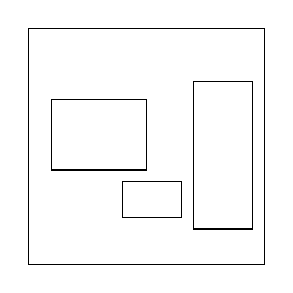
\begin{tikzpicture}[scale=.6]
\labsq{0}{0}{5}{5}{}
\labsq{.5}{2}{2.5}{3.5}{}
\labsq{2}{1}{3.25}{1.75}{}
\labsq{3.5}{.75}{4.75}{3.875}{}
\end{tikzpicture}
\end{center}
This is a $\Sigma$-free operad, via the evident insertion procedure. Note that although the three little $n$-cubes in this cofiguration were not labelled, we \emph{do} keep track of their orders.

There's a map of operads $\sigma_{n}:\scrC_n\to\scrC_{n+1}$ sending $\langle c_1,\ldots,c_j\rangle\mapsto\langle 1\times c_1,\ldots,1\times c_j\rangle$, where $1\in\Aff$ represents the identity element of $J$. Using these maps, we define $\scrC_\infty(j):=\varinjlim\scrC_n(j)$, and this inherits the structure of a $\Sigma$-free operad.
\begin{thm*}[4.8]
For $1\leq n\leq\infty$ and $j\geq1$, $\scrC_n(j)$ is $\Sigma_j$-equivariantly homotopy equivalent to the configuration space of $j$ points in $\R^n$. In particular, $\scrC_1$ is an $A_\infty$ operad, $\scrC_n$ is a locally $n-2$-connected $\Sigma$-free operad over $\calN$ for $1<n<\infty$, and $\scrC_\infty$ is an $E_\infty$ operad.
\end{thm*}

Note that the free $C_n$-algebra $C_nX$ on a space $X$ can be viewed as the configuration space of configurations of some number of disjoint little $n$-cubes in $[0,1]^n$, each labelled by a point of $X$:
\begin{center}
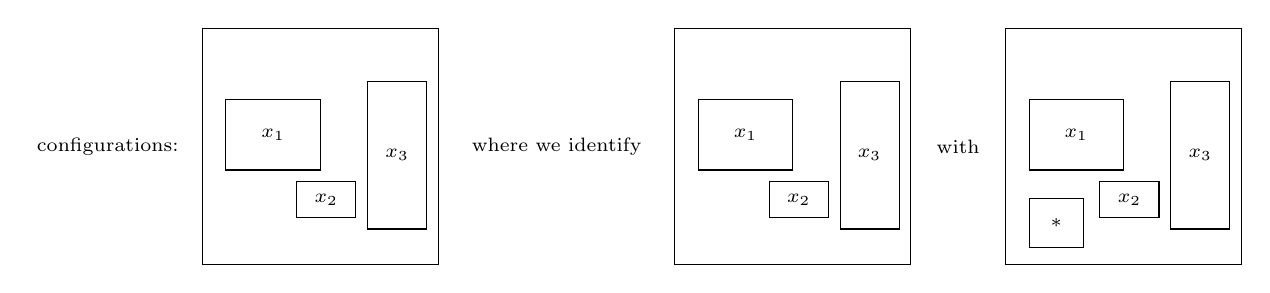
\begin{tikzpicture}[scale=.6]
\path (-2,2.5) node[font=\scriptsize] {configurations: };
\labsq{0}{0}{5}{5}{}
\labsq{.5}{2}{2.5}{3.5}{$x_1$}
\labsq{2}{1}{3.25}{1.75}{$x_2$}
\labsq{3.5}{.75}{4.75}{3.875}{$x_3$}

\path (7.5,2.5) node[font=\scriptsize] {where we identify};

\labsq[10]{0}{0}{5}{5}{}
\labsq[10]{.5}{2}{2.5}{3.5}{$x_1$}
\labsq[10]{2}{1}{3.25}{1.75}{$x_2$}
\labsq[10]{3.5}{.75}{4.75}{3.875}{$x_3$}

\path (16,2.5) node[font=\scriptsize] {with};

\labsq[17]{0}{0}{5}{5}{}
\labsq[17]{.5}{2}{2.5}{3.5}{$x_1$}
\labsq[17]{2}{1}{3.25}{1.75}{$x_2$}
\labsq[17]{3.5}{.75}{4.75}{3.875}{$x_3$}
\labsq[17]{.5}{.35}{1.65}{1.4}{$*$}
\end{tikzpicture}
\end{center}
That is, we are free to insert or remove little $n$-cubes which are labelled with the basepoint $*\in X$. Note that as we take the quotient by the symmetric group action, we \emph{no longer} need to keep track of the ordering of the cubes, only the labels.
\begin{rmk*}
We'll always draw the first coordinate of $[0,1]^n$ as the vertical direction. We'll always draw diagrams in which $n\leq2$.
\end{rmk*}
One key goal will be to prove the approximation theorem:
\begin{thm*}[2.7 --- Approximation]
If $X$ is connected, there is a weak equivalence $C_nX\to\Omega^n\Sigma^nX$.
\end{thm*}


\section{Iterated loop spaces and the \texorpdfstring{$\scrC_n$}{Cn}}
Let $\scrL_n$ be the category of $n$-fold loop spaces, for $1\leq n\leq\infty$. This category has objects sequences $\overline{Y}=\{Y_i\,|\,0\leq i\leq n\}$ such that $Y_i=\Omega Y_{i+1}$, and morphisms sequences of maps $g_i$ such that $g_i=\Omega g_{i+1}$.
\begin{itemise}
\item There is a functor $U_n:\scrL_n\to\scrT$ sending $\overline{Y}\mapsto Y_0$.
\item  There is a functor $\Omega:\scrL_n\to\scrL_{n+1}$.
\end{itemise}
\begin{thm*}[5.1]
There is a functor $\scrL_n\to\scrC_n[\scrT]$, which sends $\overline{Y}$ to $U_n\overline{Y}$, a $\scrC_n$-algebra with the evident action. Moreover, we have a commuting square:
\[\xymatrix{
\scrL_n\ar[r]\ar[d]_\Omega&\scrC_n[\scrT]\ar[d];[]_{\sigma_n^*}\\
\scrL_{n+1}\ar[r]&\scrC_{n+1}[\scrT]
}\]
\end{thm*}
We write $\theta_n$ both for the action of the operad $\scrC_n$ and of the monad $C_n$ on $U_n\overline{Y}$. Now notice that $C_\infty$, the monad associated with $\scrC_\infty$, in fact equals $\varinjlim C_n$ as a monad. The following is purely formal:
\begin{thm*}[5.2]
For $X\in\scrT$ and $1\leq n\leq\infty$, let $\alpha_n$ be the composite:
\[C_nX\overset{C_n\eta_n}{\to}C_n\Omega^nS^nX\overset{\theta_n}{\to}\Omega^nS^nX\]
Then $\alpha_n:C\nt \Omega^n S^n$ is a morphism of monads. Moreover, the following diagrams commute:
\[\xymatrix{
&\scrL_n\ar[ld]\ar[rd]\\
\Omega^n\Sigma^n[\scrT]\ar[rr]^{\alpha_n^*}&&C_n[\scrT]
}\qquad\qquad\xymatrix@C=2cm{
C_n\ar@{=>}[d]_{\sigma_n}\ar@{=>}[r]^{\alpha_n}&\Omega^{n}\Sigma^{n}\ar@{=>}[d]^{\sigma_n}\\
C_{n+1}\ar@{=>}[r]^{\alpha_{n+1}}&\Omega^{n+1}\Sigma^{n+1}
}\]
The commuting diagram of morphisms of monads (right, above) shows that we can define a monad morphism $\alpha_\infty:\Omega^\infty\Sigma^\infty\nt C_\infty$ by passage to the limit.
\end{thm*}
\section{The approximation theorem}
To prove the approximation theorem we introduce the following notions. Define a function $\Theta:\Aff\to\Aff$ which sends the affine map ``$t\mapsto x+(y-x)t$'' to 
``$t\mapsto x+(1-x)t$''. That is, $\Theta$ streches affine maps so that they reach the whole way up to 1. Write $\widetilde{\Theta}:\Aff^n\to\Aff^n$ for the function $\Theta\times1^{n-1}$. This takes a little $n$-cube and stretches it to the end of the $J^n$ in the first coordinate direction.

Suppose that $(X,A)$ is a `pair' in $\scrT$, by which we mean $A\subset X$ is a closed subset. Then we define a space $E_n(X,A)$ such that
\[C_nA\subset E_n(X,A)\subset C_nX\]
as follows. Define a function $\Psi_{A,X,n,j}:\scrC_n(j)\times X^j\to(\Aff^n)^j$ by sending
\[(\langle c_1,\ldots,c_j\rangle,x_1,\ldots,x_j)\mapsto\langle d_1,\ldots,d_j\rangle
\textup{\quad where\quad }d_i:=\begin{cases}
c_i,&\textup{if }x_i\in A;\\
\widetilde{\Theta}(c_i),&\textup{if }x_i\notin A.
\end{cases}\]
Thus $\Psi_{A,X,n,j}$ returns the little $n$-subes of a configuration, having elongated those labelled with a point outside $A$. We now define $\scrE_n(j;X,A)=\Psi_{A,X,n,j}^{-1}(\scrC_n(j))\subset \scrC_n(j)\times X^j$. One could describe this as the subset of the configurations in which no box lies over a box with a label outside $A$:
\begin{center}
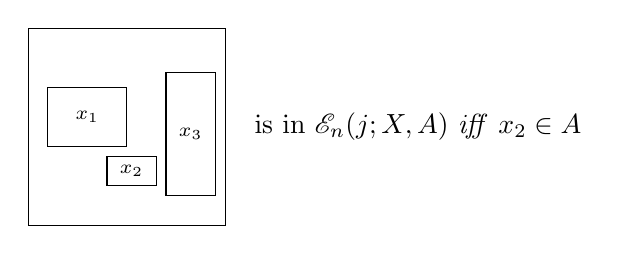
\begin{tikzpicture}[scale=.5]
\labsq{0}{0}{5}{5}{}
\labsq{.5}{2}{2.5}{3.5}{$x_1$}
\labsq{2}{1}{3.25}{1.75}{$x_2$}
\labsq{3.5}{.75}{4.75}{3.875}{$x_3$}
\path (5.5,2.5) node[right] {is in $\scrE_n(j;X,A)$ \Iff $x_2\in A$};

\end{tikzpicture}
\end{center}
Now the equivalence relation on $\coprod \scrC_n(j)\times X^j$ descends to one on  $\coprod \scrE_n(j;X,A)$, so we take the same quotient, obtaining a space $E_n(X,A)$ as advertised. Note that $E_n(X,X)=C_nX$. We might sometimes write $E_n(X):=E_n(CX,X)$, where $CX$ is the cone on $X$.
\begin{lem*}[6.7]
There is a natural surjective based map $v_n:E_n(X,*)\to C_{n-1}X$. It is defined by 
\[(\langle c_1,\ldots,c_j\rangle,x_1,\ldots,x_n)\mapsto (\langle \rho c_1,\ldots,\rho c_j\rangle,x_1,\ldots,x_n)\]
whenever $x_1,\ldots,x_n\in X\setminus\{*\}$ (every point in $E_n(X,*)$ but the basepoint can be represented in this way), where $\rho:\Aff^n\to\Aff^{n-1}$ is the projection to the last $n-1$ coordinates.
\end{lem*}
The proof of the approximation theorem depends on the following commuting diagram:
\[\xymatrix{
C_n(X)\ar[r]\ar[d]_{C_n\eta_n}&
E_n(CX,X)\ar[d]_{E_n\widetilde{\eta}_n}\ar[r]&
E_n(\Sigma X,*)\ar[r]^{v_n}\ar[d]_{E_n\eta_{n-1}}&
C_{n-1}(\Sigma X)\ar[d]_{C_n\eta_{n-1}}\\
C_n(\Omega^n\Sigma^nX)\ar[r]\ar[d]_{\theta_n}&
E_n(P\Omega^{n-1}\Sigma^nX,\Omega^{n}\Sigma^nX)
\ar[r]^{\qquad \textup{endpt}}\ar[d]_{\widetilde{\theta}_n}&
E_n(\Omega^{n-1}\Sigma^nX,*)\ar[r]^{v_n}&
C_{n-1}(\Omega^{n-1}\Sigma^nX)\ar[d]_{\theta_{n-1}}\\
\Omega^n\Sigma^nX\ar[r]&
P\Omega^{n-1}\Sigma^nX\ar[rr]^{\textup{endpt}}&&
\Omega^{n-1}\Sigma^nX
}\]
Here, the $2\times3$ block in the top left is induced by applying $E_n$ to the following commuting diagram in the category of pairs:
\[\xymatrix{
(X,X)\ar[r]\ar[d]^{\eta_n}&
(CX,X)\ar[r]\ar[d]^{\widetilde{\eta}_n}&
(\Sigma X,*)\ar[d]^{\eta_{n-1}}\\
(\Omega^n\Sigma^nX,\Omega^n\Sigma^nX)\ar[r]&
(P\Omega^{n-1}\Sigma^nX,\Omega^n\Sigma^nX)\ar[r]^{\textup{\qquad endpt}}&
(\Omega^{n-1}\Sigma^nX,*)
}\]
\textbf{Describe $\widetilde{\eta}_{n}$}. The square in the upper right hand corner is given by lemma 6.7. The maps $\theta_n$ and $\theta_{n-1}$ are given by the action of $C_n$ on an iterated loop space. Finally, we should describe $\widetilde{\theta}_n$. Suppose that $(\langle c_1,\ldots,c_j\rangle,x_1,\ldots,x_n)\in\scrE_n(j;P\Omega^{n-1}\Sigma^nX,\Omega^n\Sigma^nX)$. We will take the same example as above, in which $j=3$, and $x_2\in \Omega^n\Sigma^n X$, but $x_1,x_3$ need not be. An element of $P\Omega^{n-1}\Sigma^nX$ can be represented as a map from $[0,1]^{n}$ to $\Sigma^nX$, in which all faces but the top face are sent to the basepoint. We can produce such a map as represented by the following diagram:
\begin{center}
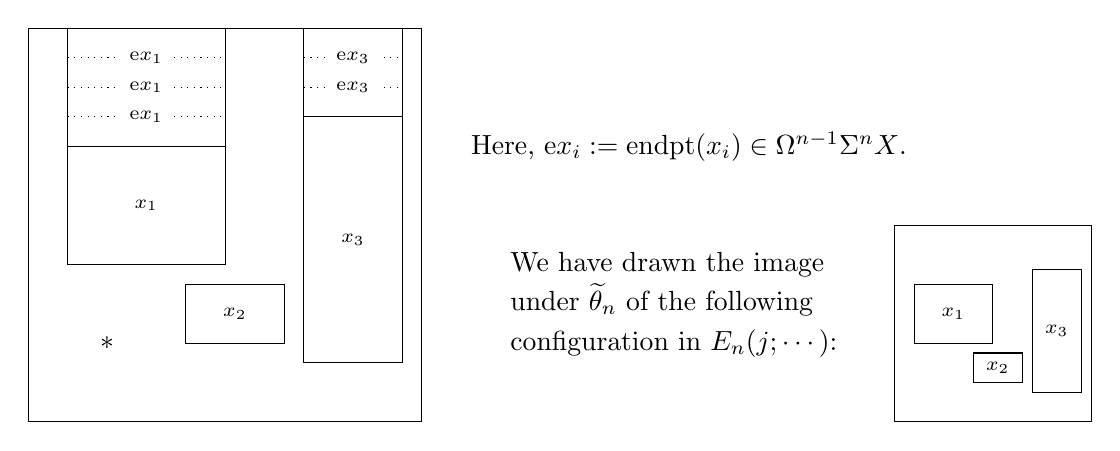
\begin{tikzpicture}
\labsq{0}{0}{5}{5}{}
\labsq{.5}{2}{2.5}{3.5}{$x_1$}
\labsq{2}{1}{3.25}{1.75}{$x_2$}
\labsq{3.5}{.75}{4.75}{3.875}{$x_3$}
\draw (.5,3) -- (.5,5);
\draw (2.5,3) -- (2.5,5);
%\draw (.5,4)--(2.5,4) node[font=\scriptsize] {g};
\path[dotted,font=\scriptsize] (.5,4.625) edge node[fill=white]{$\textup{e}x_1$} (2.5,4.625);
\path[dotted,font=\scriptsize] (.5,4.25) edge node[fill=white]{$\textup{e}x_1$} (2.5,4.25);
\path[dotted,font=\scriptsize] (.5,3.875) edge node[fill=white]{$\textup{e}x_1$} (2.5,3.875);
\draw (3.5,3.875) -- (3.5,5);
\draw (4.75,3.875) -- (4.75,5);
\path[dotted,font=\scriptsize] (3.5,4.625) edge node[fill=white]{$\textup{e}x_3$} (4.75,4.625);
\path[dotted,font=\scriptsize] (3.5,4.25) edge node[fill=white]{$\textup{e}x_3$} (4.75,4.25);
\path (1,1) node {$*$};
\path (5.5,3.5) node[right] {Here, $\textup{e}x_i:=\textup{endpt}(x_i)\in\Omega^{n-1}\Sigma^nX$.};
\path (6,2) node[right] {We have drawn the image};
\path (6,1.5) node[right] {under \smash{$\widetilde{\theta}_n$} of the following};
\path (6,1) node[right] {configuration in \smash{$E_n(j;\cdots)$}:};
\labsq[11]{0}{0}{2.5}{2.5}{}
\labsq[11]{.25}{1}{1.25}{1.75}{$x_1$}
\labsq[11]{1}{.5}{1.625}{0.875}{$x_2$}
\labsq[11]{1.75}{.375}{2.375}{1.9375}{$x_3$}
\end{tikzpicture}
\end{center}
Note that as $x_2\in\Omega^{n}\Sigma^nX$, it returns the basepoint on the entire boundary of its little $n$-cube, and we don't need to extend above it using $\textup{endpt}(x_2)$. Of course, we could not extend above that little $n$-cube, as we would collide with the cube above it.
\end{chapter4-6}
\begin{chapter7-9}
\setcounter{section}{8}
\section{A categorical construction}
\begin{itemise}
\item Homotopy in the category $s\calT$ can be defined for any category $\calT$.
\item There's an adjunction, written $\tau_*:\Hom_\calT(X,Y_0)\to\Hom_{s\calT}(X_*,Y)$:
\[\xymatrix@R=.3cm@C=2cm{
\calT  \ar@<.6ex>[r]^{(\DASH)_*}&
s\calT  \ar@<.4ex>[l]^{(\DASH)_0}\\
X \ar@{|->}[r] & X_*\makebox[0cm][l]{\,:=$\textup{const}(X)$}\\
Y_0             & Y_* \ar@{|->}[l]\\
}\]
We also have a bijection identifying maps \emph{into} the constant diagram:
\[[Y,X_*]\overset{\epsilon_*}{\from}\left\{\lambda:Y_0\to X\,\textup{\ such that\ }\,
\lambda\partial_0=\lambda\partial_1:Y_1\to X\right\}\]
\item $s$ is a 2-functor on the 2-category of categories, so that a functor $F:\calT\to\calT'$ induces a functor $F_*:s\calT\to s\calT'$ by acting levelwise, and natural transformations induce natural transformations similarly.
\item A monad $C:\calT\to\calT$ induces a monad $C_*:s\calT\to s\calT$, and $s(C[\calT])\cong C_*[s\calT]$, i.e.\ the category of simplicial $C$-algebras is the same as the category of $C_*$-algebras (whose underlying objects live in $s\calT$), by \textbf{lemma 9.3}.
\item Suppose $C:\calT\to\calT$ is a monad. A ``$C$-functor to $\calV$'' is a functor $F:\calT\to \calV$ with a right action of $C$, that is: $\lambda:FC\nt F$ satisfying unitality and associativity.
\begin{exmps*}[9.5]
Suppose $C,D:\calT\to\calT$ are monads in $\calT$ and  $\alpha:C\nt D$ is a morphism.
\begin{enumerate}\squishlist
\item $C$ itself is a $C$-functor to $\calT$. As $CT$ is naturally a $C$-algebra, $C$ can be regarded as a $C$-functor to $C[\calT]$.
\item %Let $\alpha:C\nt D$ be a morphism of monads in $\calT$.
A $\scrD$-functor $F:\calT\to\calT$ to $\calT$ (via $FD\nt F$), becomes a $\scrC$-functor to $\calT$ via the composite $FC\nt FD\nt F$.
\item[$2'$.] As $D:\calT\nt \calT$ takes values in $D[\calT]$, it can be taken as a $C$-functor to $D[\calT]$ via the map $DC\nt DD\nt D$. It can also then be viewed as a $C$-functor to $C[\calT]$. Moreover, $\alpha:\scrC\nt\scrD$ is a morphism of $\scrC$-functors to $C[\calT]$.
\item Suppose we have an adjunction $\xymatrix@R=.3cm{
\calT  \ar@<.6ex>[r]^{\Sigma}&
\calV  \ar@<.4ex>[l]^{\Lambda}}$, giving a monad $\Lambda\Sigma$ in $\calT$. Then $\Sigma$ is a $\Lambda\Sigma$-functor to $\calV$, via $\Sigma\Lambda\Sigma\nt \id\Sigma=\Sigma$.
\item Suppose we have an morphism $\alpha:C\nt\Lambda\Sigma$ of monads in $\calT$. Taking adjoints, we obtain a natural transformation $\alpha':\Sigma C\nt \Sigma$ of functors $\calT\to\calV$, which gives $\Sigma$ the structure of $\scrC$-functor to $\calV$. 
\item[$4'$.] The morphism $\alpha$ of monads induces a morphism $C\nt\Lambda\Sigma$ of $C$-functors to $C[\calT]$.
\end{enumerate}
\end{exmps*}
\subsection*{The categorical 2-sided bar construction}
Let $\calB(\calT,\calV)$ be the category whose objects are triples $(F,C,X)$, where $C$ is a monad in $\calT$, $X$ is a $C$-algebra (in $\calT$), and $F$ is a $C$-functor to $\calV$. Define a functor
\[B_*:\calB(\calT,\calV)\to s\calV\textup{\quad by\quad}B_q(F,C,X)=FC^qX\]
There are $q+1$ different `action maps' with which to form a map $FC^qX\to FC^{q-1}X$: 
\begin{itemise}
\item the right action of $C$ on $F$ induces $\partial_0$;
\item the $n-1$ different multiplications on $C$ induce $\partial_i$ for $1\leq i\leq n-1$;
\item the left action of $C$ on $X$ induces $\partial_q$.
\end{itemise}
Moreover, there are $n+1$ different positions to insert the unit of $C$, giving the maps $s_i$ for $1\leq i\leq n$. Thus we have actually define a functor to $s\calV$, the \emph{categorical two-sided bar construction}.
\begin{itemize}\squishlist
\item \textbf{Lemma 9.7:} Suppose that $G:\calV\to\calV'$ is a functor. Then $GF:\calT\to\calV'$ is a $C$-functor, and for an $C$-algebra $X$:
\[B_*(GF,C,X)=G_*B_*(F,C,X).\]
\item \textbf{Proposition 9.8:} $X_*$ is a strong deformation retract of $B(C,C,X)$ in $s\calT$.
\item \textbf{Proposition 9.9:} $F_*Y_*$ is a strong deformation retract of $B(F,C,CY)$ in $s\calT$.
\item \textbf{Theorem 9.10:} 
Suppose $C,D:\calT\to\calT$ are monads, and  $\alpha:C\nt D$ is a morphism.
\begin{enumerate}\squishlist
\item If $X$ is a $C$-algebra, we have a compatibility, as in the left diagram:
\[\xymatrix@C=1.8cm{
\ar@{=}[d]X_*&\ar[l]_{\epsilon_*(\xi)\qquad}^{\textup{sdr\qquad}}
B_*(C,C,X)\ar[r]^{B_*(\alpha,1,1)}
&B_*(D,C,X)\\
X_*\ar[ur]_(.8){\tau_*(\eta)}\ar[urr]_(.8){\tau_*(\zeta)}&
&\makebox[0cm][c]{(in $sC[\calT]$)}
}\qquad\vrule\qquad\xymatrix@C=.5cm{
X\ar@{=}[d]&\ar[l]_{\xi}CX\ar[r]^\alpha&DX\\
X\ar[ur]_(.8){\eta}\ar[urr]_(.8){\zeta}&&\makebox[0cm][c]{(in $\calT$)}
}\]
Here, recall that $\tau_*$ is the adjunction, so that $\tau_*(\eta)$ is the adjoint of the map $\eta:X\to CX=B_0(C,C,X)$ induced by the unit of $C$. Also, the strong deformation retract $\epsilon_*(\xi):B_*(C,C,X)\to X_*$ is the image of the action map $\xi:B_0(C,C,X)=CX\to X$ under $\epsilon_*$. This is indicated by the right hand diagram.
\item If $X$ is a $D$-algebra via $\xi':DX\to X$, then $X$ is also a $C$-algebra, via $\xi'\alpha$. We can then extend the above as follows:
\[\xymatrix@C=1.8cm{
\ar@{=}[d]X_*&\ar[l]_{\epsilon_*(\xi'\alpha)\quad}^{\textup{sdr\qquad}}
B_*(C,C,X)\ar[r]^{B_*(\alpha,1,1)}
&B_*(D,C,X)\ar@/_1cm/[ll]^{\epsilon_*(\xi')}\\
X_*\ar[ur]_(.8){\tau_*(\eta)}\ar[urr]_(.8){\tau_*(\zeta)}&&\makebox[0cm][c]{(in $sD[\calT]$)}
}\qquad\vrule\qquad\xymatrix@C=.5cm{
X\ar@{=}[d]&\ar[l]_{\xi'\alpha}CX\ar[r]^\alpha&DX\ar@/_1cm/[ll]^{\xi'}\\
X\ar[ur]_(.8){\eta}\ar[urr]_(.8){\zeta}&&\makebox[0cm][c]{(in $\calT$)}
}\]
\item If $Y\in\calT$, $CY$ is a $C$-algebra, $DY$ is a $D$-algebra, and:
\[\xymatrix@C=1.8cm{
\ar@{=}[d]D_*Y_*&\ar[l]_{\epsilon_*(\nu\circ D\alpha)\qquad}^{\textup{sdr\qquad}}
B_*(D,C,CY)\\
D_*Y_*\ar[ur]_(.8){\tau_*(D\eta)}
&\makebox[0cm][c]{(in $sD[\calT]$)}
}\qquad\vrule\qquad\xymatrix@C=.5cm{
DY\ar@{=}[d]&\ar[l]_{\nu}DDY&\ar[l]_{D\alpha}DCY\\
DY\ar[urr]_(.8){D\eta}&&\makebox[0cm][c]{(in $\calT$)}
}\]
\end{enumerate}
\item \textbf{Theorem 9.11:} 
Suppose that we have a monad $C$ in $\calT$, an adjunction 
$\xymatrix{
\Sigma:\calT  \ar@<.6ex>[r]&
\calV:\Lambda  \ar@<.4ex>[l]
}$, giving a monad $\Lambda\Sigma$ in $\calT$, and a map $\alpha:C\nt \Lambda\Sigma$ of monads:
\UseAllTwocells
\[\xymatrix@R=.2cm{
\calT\ar[dd]_C\ar[dr]^\Sigma&\\
&\calV\ar[dl]^\Lambda\\
\calT\uutwocell\omit{<3>}
}\]
We can de-$\Lambda$ the following bar constructions:
\begin{itemize}\squishlist
\item[2.] $B_*(\Lambda\Sigma,C,\Lambda \DASH):\calV\to s\calT$ [note that for $Y\in\calV$, $\Lambda Y$ is a $\Lambda\Sigma$-algebra via the counit of the adjunction, and thus a $C$-algebra].
\item[3.] $B_*(\Lambda\Sigma,C,C\DASH):\calT\to s\calT$.% for $Y\in\calT$.
\end{itemize}
That is we'll have commuting diagrams of functors:
\[\xymatrix{
 \calV\ar[rr]^{B_*(\Lambda\Sigma,C,\Lambda\DASH)}\ar[dr]_{B_*(\Sigma,C,\Lambda\DASH)}& & s\calT& &\calT\ar[rr]^{B_*(\Lambda\Sigma,C,C\DASH)}\ar[dr]_{B_*(\Sigma,C,C\DASH)}& & s\calT\\
& s\calV\ar[ur]_{\Lambda^*}&&&& s\calV\ar[ur]_{\Lambda^*}
}\]
\begin{itemize}\squishlist
\item[2.] We are in a similar situation as in 9.10.2, with $D=\Lambda\Sigma$ and $X=\Lambda Y$. All we have to add here is that the curvy map from above is not only induced by a map in $\calT$, as before, but now from the counit ``$\textup{cu}$'', a map in $\calV$:
\[\xymatrix@C=1.4cm{
\Lambda_*Y_*&B_*(\Lambda\Sigma,C,\Lambda Y)\ar@/_.4cm/[l]^{\Lambda_*\epsilon_*(\textup{cu})\quad}
}\quad\vrule\quad\xymatrix@C=1.4cm{
Y_*&B_*(\Sigma,C,\Lambda Y)\ar@/_.4cm/[l]^{\epsilon_*(\textup{cu})\quad}
}\quad\vrule\quad\xymatrix@C=1.4cm{
Y&\Sigma\Lambda Y\ar@/_.4cm/[l]^{\textup{cu}}
}\]
\item[3.] Now we're as in 9.10.3, and can de-$\Lambda$ the whole retraction diagram. Let $\alpha^\textup{T}:\Sigma C\nt\Sigma$ be adjoint to $\alpha: C\nt\Lambda\Sigma$, then we have:
\[\xymatrix@C=1.5cm{
\ar@{=}[d]\Lambda_*\Sigma_*Y_*&
\ar[l]_{\Lambda_*\epsilon_*(\Sigma\alpha^\textup{T})\qquad}^{\textup{sdr\qquad}}
B_*(\Lambda\Sigma,C,CY)\\
\Lambda_*\Sigma_*Y_*\ar[ur]_(.8){\Lambda_*\tau_*(\Sigma\eta)}
&\makebox[0cm][c]{(in $s\Lambda\Sigma[\calT]$)}
}\ \vrule\ \xymatrix@C=1.3cm{
\ar@{=}[d]\Sigma_*Y_*&
\ar[l]_{\epsilon_*(\Sigma\alpha^\textup{T})\qquad}^{\textup{sdr (!)\qquad}}
B_*(\Sigma,C,CY)\\
\Sigma_*Y_*\ar[ur]_(.8){\tau_*(\Sigma\eta)}
&\makebox[0cm][c]{(in $s\Sigma[\calT]$)}
}\ \vrule\ \xymatrix@C=1cm{
\ar@{=}[d]\Sigma Y&
\ar[l]_{\Sigma\alpha^\textup{T}}
\Sigma CY\\
\Sigma Y\ar[ur]_(.8){\Sigma\eta}
&\makebox[0cm][c]{(in $\calT$)\quad}
}\]
\end{itemize}
%Note further that $B_*(\Lambda\Sigma,C,\Lambda Y)=\Lambda_*B_*(\Sigma,C,\Lambda Y)$, so the construction can be de-$\Lambda$-fied, at least on objects.
\end{itemize}
\end{itemise}
\end{chapter7-9}
\end{document}
















